\documentclass[11pt,a4paper]{article}

\usepackage[margin=0.85in]{geometry}
\usepackage[T1]{fontenc}
\usepackage{lmodern}
\usepackage{microtype}
\usepackage{setspace}
\usepackage{enumitem}
\usepackage{booktabs}
\usepackage{array}
\usepackage{tikz}
\usetikzlibrary{arrows.meta,positioning,shapes.geometric,fit,calc}
\usepackage{titlesec}
\usepackage{caption}
\usepackage{graphicx}
\usepackage[hidelinks]{hyperref}

\setstretch{1.03}
\setlength{\parindent}{0pt}
\setlength{\parskip}{4pt}
\setlist[itemize]{leftmargin=1.45em,itemsep=1pt,topsep=2pt}
\setlist[enumerate]{leftmargin=1.55em,itemsep=1pt,topsep=2pt}

\titleformat{\section}{\Large\bfseries}{\thesection}{0.65em}{}
\titleformat{\subsection}{\large\bfseries}{\thesubsection}{0.65em}{}
\titleformat{\subsubsection}{\normalsize\bfseries}{\thesubsubsection}{0.65em}{}
\titlespacing*{\section}{0pt}{10pt}{3pt}
\titlespacing*{\subsection}{0pt}{7pt}{2pt}
\titlespacing*{\subsubsection}{0pt}{6pt}{2pt}

\tikzset{
 box/.style={draw,rounded corners=2pt,align=center,minimum height=0.7cm,
             minimum width=2.5cm,font=\small,fill=blue!5},
 arrow/.style={-{Latex[length=2mm]},thick},
}

\begin{document}

% ---------------- Title Page ----------------
\begin{center}
{\LARGE\bfseries HyperTrack: Hyperhidrosis Monitoring and Management System\par}
\vspace{3pt}
{\large A Web-Based Self-Reporting, Trigger-Awareness, and AI-Assisted Tracking Tool\par}
\vspace{6pt}
{\large Project Report: Prototype Stage, UCS503P\par}
{\large Submitted to: Dr. Jeelani Asif\par}
\vspace{10pt}

\includegraphics[height=2.6cm]{tiet-logo-red.png}

\vspace{4pt}
{\large\bfseries THAPAR INSTITUTE\par}
{\small OF ENGINEERING \& TECHNOLOGY\par}
{\small (Deemed to be University)\par}
\vspace{12pt}

\begin{tabular}{cc}
\textbf{Prabhkirat Kaur, AIML} & \textbf{Aditya Rajput, AIML} \\
\small\href{mailto:pkaur_be24@thapar.edu}{pkaur\_be24@thapar.edu} &
\small\href{mailto:arajput_be24@thapar.edu}{arajput\_be24@thapar.edu} \\
\small Roll No: 1024240024 & \small Roll No: 1024240145 \\
\end{tabular}

\vspace{6pt}
{\normalsize September 14, 2026\par}
\end{center}

\vspace{6pt}
\tableofcontents

\clearpage

\section{Introduction}

\subsection{Background and Context}
Hyperhidrosis (primary focal hyperhidrosis) is a dermatological condition characterised by
uncontrollable, excessive sweating well beyond physiological thermoregulatory needs,
predominantly affecting the palms, soles, axillae, and craniofacial regions. Patients living
with the condition frequently report psychosocial distress and impairment in daily
professional and social functioning.

A recurring obstacle during dermatological consultations is \emph{retrospective recall bias}:
patients are asked to summarise how often episodes occur, when they peak during the day, and
what triggers them (stress spikes, ambient temperature, caffeine, physical activity), but
without a structured log this is largely guesswork. Clinicians end up making judgements from an
incomplete, self-reported history rather than from consistent, timestamped data.

\subsection{Problem Statement}
Given that patients have no structured way to log individual sweating episodes as they happen,
we want a system that lets a patient (i) record an episode in under a minute with the details
that matter clinically (severity, duration, body area, trigger, stress level, activity,
environmental conditions), (ii) see their own frequency and trigger patterns on a live
dashboard between visits, and (iii) get a plain-language, AI-generated summary of their own
history that is grounded in what they actually logged, not a generic sweating FAQ.

\subsection{Project Objectives}
\begin{enumerate}
    \item \textbf{Objective 1:} Build an authenticated, real-time episode-logging pipeline —
    from a validated client-side form, through secure per-user storage, to a live dashboard —
    so a logged episode is reflected in the user's own statistics immediately, without a manual
    refresh.
    \item \textbf{Objective 2:} Add an AI layer, strictly scoped to a single user's own logged
    episodes, that produces (a) a natural-language insights summary with key patterns and
    preventative tips, and (b) a conversational assistant that answers the user's questions
    grounded in that same history, rather than a general LLM answer about hyperhidrosis in
    the abstract.
    \item \textbf{Objective 3:} Ship a usable, patient-facing web application (login, log
    episode, dashboard, history, analytics, reports) that a real person could operate without
    training, as the demoable surface for the above two objectives.
\end{enumerate}

These objectives are achievable within a single semester because the scope is deliberately
bounded to a single-user tracking and insights tool (no clinician-facing portal, no diagnosis
or treatment logic), built on managed services (Firebase, a hosted LLM API) rather than
infrastructure we would otherwise have to build and operate ourselves.

\vspace{2pt}
\noindent\fbox{\parbox{\dimexpr\linewidth-2\fboxsep-2\fboxrule}{
\textbf{Clinical scope boundary:} HyperTrack is strictly an observation and self-documentation
aid. It does not diagnose hyperhidrosis or any other condition, and does not prescribe
treatment. Every AI-generated response explicitly directs the user to consult a licensed
dermatologist for medical decisions.
}}

\section{Methodology and Design}

\subsection{System Architecture}

\subsubsection{High-Level Design}
The system is a two-tier web application. A React single-page application is the only surface
the patient interacts with; it talks to two backing services. Authentication and all episode
data go directly from the browser to \textbf{Firebase} (Authentication + Cloud Firestore) using
the Firebase client SDK — there is no custom database or server-side CRUD layer for this part.
A small \textbf{FastAPI} service sits alongside it purely to keep the Gemini API key off the
client and to host the two AI endpoints (insights generation and contextual chat). The frontend
never talks to Gemini directly.

\begin{figure}[h!]
\centering
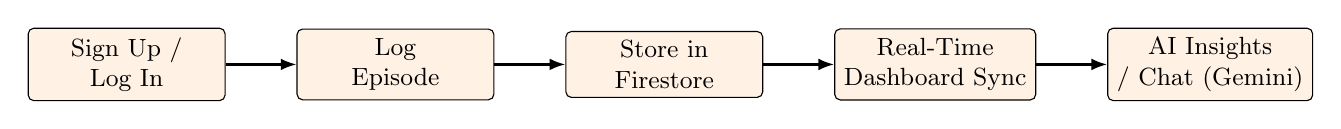
\begin{tikzpicture}[node distance=0.55cm and 0.9cm]
\node[box,fill=orange!10] (a) {Sign Up /\\Log In};
\node[box,right=of a,fill=orange!10] (b) {Log\\Episode};
\node[box,right=of b,fill=orange!10] (c) {Store in\\Firestore};
\node[box,right=of c,fill=orange!10] (d) {Real-Time\\Dashboard Sync};
\node[box,right=of d,fill=orange!10] (e) {AI Insights\\/ Chat (Gemini)};
\draw[arrow] (a) -- (b);
\draw[arrow] (b) -- (c);
\draw[arrow] (c) -- (d);
\draw[arrow] (d) -- (e);
\end{tikzpicture}
\caption{End-to-end data flow: authentication, episode logging, Firestore persistence,
real-time sync to the dashboard/history/analytics views, and on-demand AI insights/chat.}
\end{figure}

If a Firestore write for a new episode succeeds, every open view subscribed to that user's
episode collection (Dashboard, History, Analytics) is pushed the update automatically through a
real-time listener (\texttt{onSnapshot}) — there is no polling. AI Insights and AI Chat are
pulled on demand: the frontend sends the user's episode list (and, for chat, the question) to
the FastAPI backend, which prompts Gemini and returns a structured response.

\begin{figure}[h!]
\centering
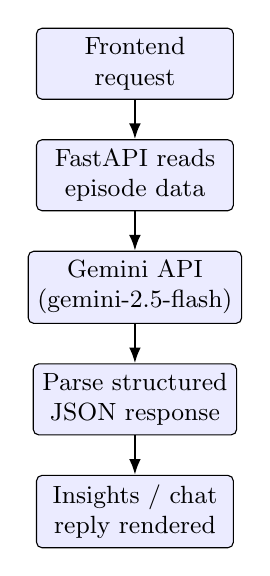
\begin{tikzpicture}[node distance=0.5cm and 0.9cm]
\node[box,fill=blue!8] (req) {Frontend\\request};
\node[box,below=of req,fill=blue!8] (fast) {FastAPI reads\\episode data};
\node[box,below=of fast,fill=blue!8] (gem) {Gemini API\\(gemini-2.5-flash)};
\node[box,below=of gem,fill=blue!8] (parse) {Parse structured\\JSON response};
\node[box,below=of parse,fill=blue!8] (out) {Insights / chat\\reply rendered};
\draw[arrow] (req) -- (fast);
\draw[arrow] (fast) -- (gem);
\draw[arrow] (gem) -- (parse);
\draw[arrow] (parse) -- (out);
\end{tikzpicture}
\caption{AI Insights / Chat workflow: the backend never lets Gemini see any user's data other
than the requester's own, and always returns a structured (not free-form) response so the
frontend can render it reliably.}
\end{figure}

\subsubsection{Technical Stack}
\begin{itemize}
    \item \textbf{Frontend:} React 19, TypeScript, Vite, Tailwind CSS 4, React Router 7.
    \item \textbf{Auth \& Database:} Firebase Authentication (email/password) and Cloud
    Firestore, queried in real time via \texttt{onSnapshot} listeners filtered by \texttt{userId}.
    \item \textbf{AI Backend:} FastAPI + Uvicorn, Firebase Admin SDK (for backend-side trust),
    Pydantic for request/response models.
    \item \textbf{AI Model:} Google Gemini (\texttt{gemini-2.5-flash}, with fallback handling
    for newer Gemini model names) via the \texttt{google-genai} client — used purely as a hosted
    reasoning/summarisation layer over data the user already owns; no model is trained by us.
    \item \textbf{Dev tooling:} Vite dev-server proxy (\texttt{/api/*} $\to$
    \texttt{localhost:8000}) to avoid CORS friction locally; \texttt{oxlint} for frontend
    linting.
\end{itemize}

\subsection{Implementation Details}
The implementation is split across three logical modules, developed and reviewed jointly by
both team members.

\subsubsection{Module 1: Frontend \& Authentication}
This module owns the React SPA shell: routing, the \texttt{AuthContext} (tracks the current
Firebase user across the app), and \texttt{ProtectedRoute} (redirects to \texttt{/login} if no
session exists). It also owns the episode-logging form (\texttt{LogEpisode.tsx}), which
performs client-side validation — a severity rating, at least one affected body area, and a
duration are required before the form will submit — before handing a validated object to the
data layer.

\subsubsection{Module 2: Data Layer \& Real-Time Sync}
This module (\texttt{services/episodes.ts}) wraps all Firestore access: writing a new episode
document (tagged with \texttt{userId} and a server timestamp), and subscribing the Dashboard,
History, and Analytics pages to that user's \texttt{episodes} collection via
\texttt{onSnapshot}. Aggregate statistics shown on these pages (average severity, top trigger,
body-area distribution, severity buckets) are computed client-side in React from the live
snapshot rather than being pre-computed and stored — there is no separate analytics service.

\subsubsection{Module 3: AI Backend (FastAPI + Gemini)}
This module (\texttt{code/backend/app/routers/ai.py}) exposes two endpoints. \texttt{POST
/api/ai/insights} accepts a user's episode list and returns a structured JSON object
(\texttt{summary}, \texttt{keyPatterns}, \texttt{preventativeTips}) generated by Gemini.
\texttt{POST /api/ai/chat} accepts a free-text question plus the same episode list as context,
so the model's answer is grounded in that specific user's history rather than being a generic
response about hyperhidrosis. If the user has zero logged episodes, the insights endpoint
returns a friendly placeholder message instead of calling Gemini at all, and any Gemini/API
failure is surfaced to the frontend as a clear error rather than failing silently.

\section{Results and Evaluation}

\subsection{Testing Methodology}
\begin{itemize}
    \item \textbf{Manual functional testing:} Every screen (Login, Log Episode, Dashboard,
    History, Analytics, AI Insights, AI Chat) has been manually exercised end to end against a
    live Firebase project, including the real-time update path (logging an episode in one tab
    and confirming the Dashboard in another tab updates without a refresh).
    \item \textbf{Backend smoke test:} \texttt{code/backend/test\_insights.py} is a small script
    that posts a sample request to \texttt{/api/ai/insights} and confirms a \texttt{200}
    response with a well-formed body. This is a manual smoke check, not yet an automated
    \texttt{pytest} suite.
    \item \textbf{Not yet carried out at the prototype stage:} automated unit/integration tests
    for the frontend or backend, load/performance testing, and a structured usability study with
    users outside the team. These are explicitly scoped into Section~3.2 and Section~4.3 rather
    than left unstated.
\end{itemize}

\subsection{Analysis}
At the prototype stage, our goal was to prove the full loop works end to end on a live backend
— login, log an episode, see it reflected instantly across every view, and get an AI-generated
summary of the resulting history — rather than to report accuracy numbers, since there is no
model of our own being evaluated (Gemini is used as-is via API). On that front we are on track:
authentication, real-time Firestore sync, and both Gemini-backed endpoints all function against
the deployed Firebase project described in Section~2.1.2.

We are deliberately flagging one known gap rather than glossing over it: the Dashboard's ``AI
Pattern Intelligence'' card currently displays a static, hardcoded confidence figure
(\texttt{94.2\%}) that is \emph{not} computed from real data — it is placeholder UI text left
over from early design work, whereas the actual AI Insights and Chat pages do make a live,
data-grounded call to Gemini. We would rather report this honestly now than have it surface
unexpectedly during evaluation; it is tracked as the first item in Section~4.3.

The main engineering challenge so far has been keeping the Firestore query shape (filtering
every read by \texttt{userId}, and choosing which fields to denormalise for the Analytics
page) consistent between the logging form and the three read views, since a mismatch there
silently produces an empty or incorrect dashboard rather than a visible error. We addressed
this by centralising all Firestore access in a single \texttt{services/episodes.ts} module
instead of duplicating queries per page.

\section{Conclusion}

\subsection{Summary of Work}
At this stage we have a working prototype covering the full patient-facing loop: Firebase
authentication with protected routing, a validated episode-logging form, real-time
Firestore-backed Dashboard/History/Analytics views, and a FastAPI + Gemini backend for AI
Insights and AI Chat, both grounded in the requesting user's own data. Of our three objectives,
the first (real-time logging pipeline) and third (usable end-to-end application) are
functionally complete and demoable; the second (AI layer) is functionally in place for
Insights and Chat, with the one known placeholder metric noted above still to be resolved.

\subsection{Key Findings}
\begin{itemize}
    \item \textbf{Finding 1:} Using Firestore's real-time listeners instead of manual polling
    or a custom backend for CRUD meant the ``data freshness'' requirement (dashboard reflects a
    new episode instantly) came essentially for free, rather than needing a websocket layer we
    would have had to build ourselves.
    \item \textbf{Finding 2:} Keeping Gemini strictly scoped to one user's own episode data —
    both for Insights and Chat — and never exposing the API key to the browser, gave us a clean
    security boundary with very little extra code (one FastAPI router).
    \item \textbf{Finding 3:} Splitting responsibilities as ``Firebase owns data + auth,
    FastAPI owns only AI'' kept the two halves of the system independently testable: the core
    app is fully usable even if the AI backend is not running, which was useful while developing
    the two halves in parallel.
\end{itemize}

\subsection{Future Work and Recommendations}
\begin{enumerate}
    \item Replace the hardcoded \texttt{94.2\%} ``Model Confidence'' figure on the Dashboard
    with either a genuinely computed metric or remove it, so every number shown to the user is
    backed by real data.
    \item Add an automated test suite: component/unit tests for the episode-validation logic
    and Firestore query helpers on the frontend, and a proper \texttt{pytest} suite (beyond the
    current manual smoke script) for the FastAPI endpoints.
    \item Implement the Reports page's CSV/PDF export server-side (currently browser-rendered
    only), so a user can share a clean report with a physician outside the app.
    \item Run a small structured usability pass with users outside the team on the logging
    form and AI Chat, and use that feedback to prioritise final-stage UX changes.
    \item Longer term, evaluate whether a lightweight, locally-computed statistical
    "confidence" or trend-significance measure could genuinely back an insights-confidence
    indicator, rather than relying solely on Gemini's qualitative summary.
\end{enumerate}

\subsection{Final Remarks}
Building this prototype clarified the difference between ``the app looks AI-powered'' and ``the
app's AI feature is actually grounded in the user's own data'' — a distinction we now treat as
a hard requirement rather than a nice-to-have, which is also why we are reporting the one
placeholder metric honestly instead of leaving it to be discovered later. We are satisfied with
where the prototype stands: the core logging-and-dashboard loop and both Gemini-backed features
work end to end against a live backend, and the remaining work before final submission is
focused on testing rigour, the export feature, and resolving the one flagged UI placeholder.

\end{document}
